In this chapter, we will introduce the RoboCup Soccer 3D domain, where all experiments will be conducted. Furthermore, we will introduce the principles of a keyframe movement and optimization techniques. Finally, we will review the literature regarding Reinforcement Learning for control tasks.

\section{The RoboCup Soccer 3D Simulation League}
\subsection{Domain Description}
The RoboCup Soccer 3D Simulation League (Soccer 3D) is a particularly interesting challenge concerning humanoid robot soccer. It consists of a simulation environment for a soccer match with two teams, each one composed by up to 11 simulated Nao robots \cite{gouaillier2009}, the official robot used for the RoboCup Standard Platform League since 2008. The Soccer 3D is interesting for robotics research, since it involves high level multi-agent cooperative decision making, while providing a physically realistic environment, which requires control and signal processing techniques for robust low level skills.

The RoboCup 3D simulation environment is based on SimSpark \cite{simspark}, a generic
physical multi-agent system simulator. SimSpark uses the Open Dynamics Engine (ODE) library for its realistic simulation of rigid body dynamics with
collision detection and friction. The Nao robot has height of approximately 57 cm and 4.5 kilograms. The agent send speed commands to the simulator and receive perceptual data. Each robot has 22 joints with perceptors and effectors. Communication between agent and server happens in the frequency of 50 Hz \cite{AAAI12-MacAlpine}. 

\subsection{ Kick Motion }
In the current level of the Soccer 3D evolution, motion control is a key factor in team's performance. Indeed, controlling a high degrees of freedom humanoid robot is acknowledged as one of the hardest problems in Robotics. Much effort has been devised to humanoid robot walking, where researchers have been very successful in designing control algorithms which reason about reduced order mathematical models based upon the Zero Moment Point (ZMP) concept, such as the linear inverted pendulum model \cite{kajita2001}. Nevertheless, these techniques restrict the robot to operate under a small region of its dynamics, where assumptions of the simplified models are still valid \cite{collins2005,muniz2016}.

Therefore, model-based techniques are hard to use for designing highly dynamic movements, such as long distance kicks and goalkeeper dives to defend goals from fast moving balls. In the robot soccer domain, a common approach for these movements is to employ keyframe movements, where motions are composed by sequences of robot postures. In this case, movements are designed off-line and executed in an open-loop fashion in execution time.

Due to the lack of mathematical models, an approach frequently employed is to rely on human intuition to design keyframe movements by hand, usually aided by graphical tools. However, this process is difficult, time consuming, and is often unable to obtain high performance motions given the high dimensionality of the search space. Other possible solution is to use motion capture from humans \cite{shon2005}, which has its own challenges due to the fact that the kinematic and dynamic properties of a humanoid robot differs greatly from those of a human.

\subsection{Keyframe Movements}\label{sec:keyframe-movements}

\begin{definition}
A \emph{keyframe} \( \mathrm{\mathbf{k}} = \left[ j_1, j_2, \dots, j_n \right]^T \in K \subseteq \mathbb{R}^n \) is an ordered set of joint angular positions, where \( K \) and \( n \) are the joint space and the number of degrees of freedom of the robot.
\end{definition}

\begin{definition}
A \emph{keyframe step} is an ordered pair \( \mathrm{\mathbf{s}} = \left( \mathrm{\mathbf{k}}, t \right) \in S = K \times \mathbb{R} \), where \( \mathrm{\mathbf{k}} \) is a keyframe and \( t \) is the time when the keyframe must be achieved with respect to the beginning of the movement. 
\end{definition}

\begin{definition}{break}
A \emph{keyframe movement}, or simply a movement, is defined as \( \mathrm{\mathbf{m}} = \left( \mathrm{\mathbf{s}}_1, \mathrm{\mathbf{s}}_2, \dots, \mathrm{\mathbf{s}}_{\gamma}, r \right) \in M = S^{\gamma} \times \mathbb{R} \), where \( \gamma \) and \( r \) are the number of keyframe steps and the speed rate of the movement. In this representation, we assume the movement starts at time 0 and the first keyframe step represents the robot posture at the beginning of the movement. Therefore, \( t_1 = 0 \) and each time \( t_i, \forall i \geq 2 \) is a time since the beginning of the movement.
\end{definition}

Keyframe movements are executed in an open-loop fashion, where joint positions are computed through interpolation of keyframe steps based upon the current time. If the interface to the robot joints is not position-based, local controllers may be used to track the position references issued by the keyframe. For example, in the Simspark simulator, the simulated Nao Robot has speed-controlled joints, therefore, we use simple proportional controllers for each joint to track desired joint positions. To obtain smooth joint trajectories, we interpolate keyframe steps, by using cubic splines \cite{bartels1987}, which are functions of class \( \mathcal{C}^2 \). 

Finally, when a keyframe movement is requested, joint positions are often far away from movement's initial joint positions. Hence, simply executing the keyframe movement in this case would result in high joints accelerations, which would probably make the robot to fall. To avoid this from happening, a transition movement based on linear interpolation is first employed to bring the joint positions to the initial joint positions required by the keyframe movement.

\subsection{Optimization Techniques}

In Soccer 3D environment, optimization techniques plays a important role to achieve competitive behaviors, because they are used to obtain faster and more robust motions.

Motion optimization means finding the best values for each joint in the time instant during the whole motion. There's a lot of parameters involved, which makes manual tuning impossible. The common way to do this is parameterizing the motion and using optimization algorithms to find the best parameters for this model. For the kick motion, it means find the best keyframe and interpolator values. In the case of walking motion, there is a analytical control algorithm based upon Zero Moment Point (ZMP) and we optimize the walk parameters used in this algorithm, such as torso height, period and step size.

In the robotics simulation world, it's common to optimize using evolution strategies. \citeauthor{tgmaximo} used Particle Swarm Optimization to optimize walk parameters. \cite{AAMAS11-urieli} compared the performance of several algorithms in Soccer 3D context, such as Hill Climbing (HC), Cross-Entropy Method (CEM) \cite{Rubinstein:2004:CEM:1014902}, Genetic Algorithm and Covariance Matrix Adaptation Evolution Strategy (CMA-ES) \cite{cmaes}. The latter proved to be the most successful within the Soccer 3D environment in optimizing walking and kicking \cite{AAAI12-MacAlpine} \cite{AAMAS11-urieli}, therefore being the most common in this environment. 

\begin{figure}[ht!]
	\centering
	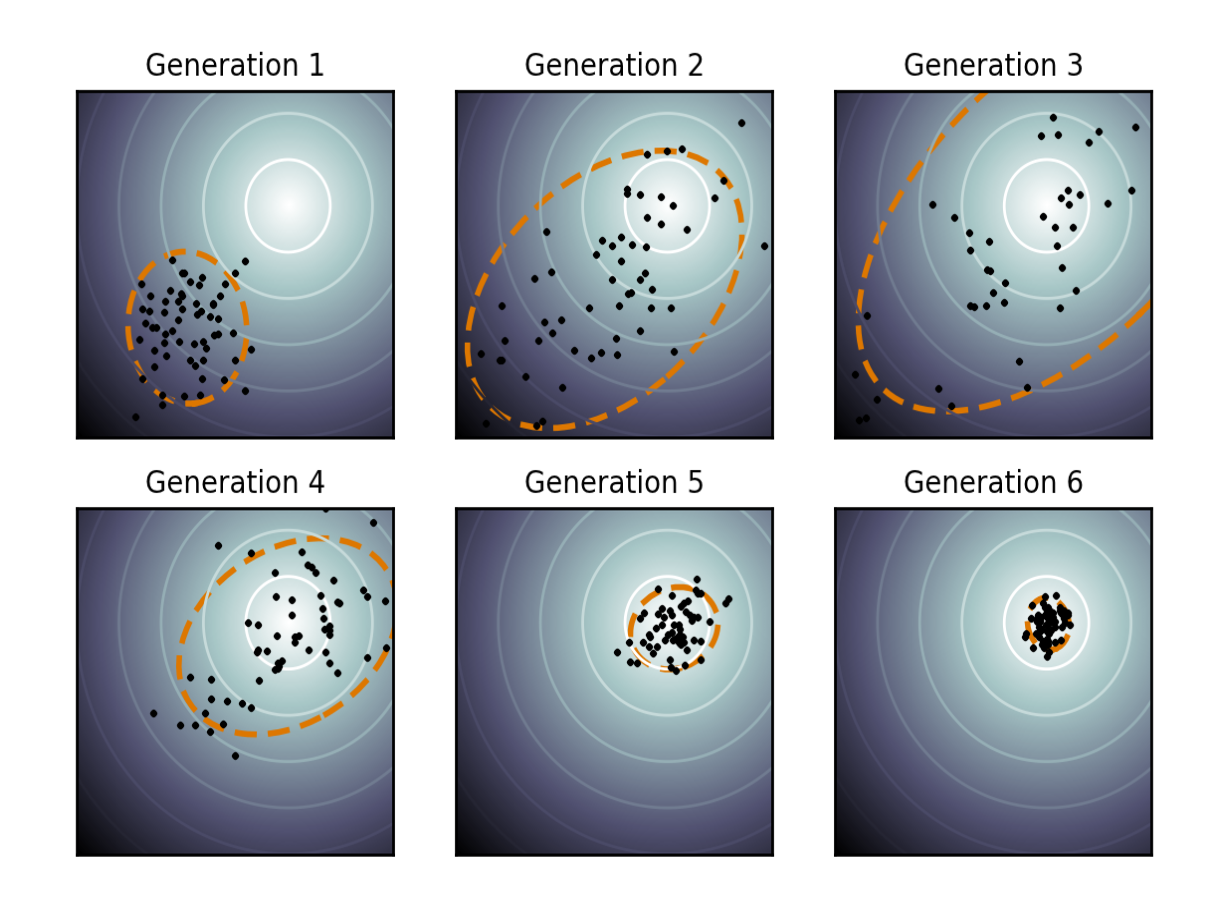
\includegraphics[width=0.8\textwidth]{Cap2/CMAES.eps}
	\caption{Illustration of an actual optimization run with covariance matrix adaptation on a simple two-dimensional problem
		\cite{cmaesfig}.}
	\label{cmaesfigure}
\end{figure}

The CMA-ES algorithm is a policy search algorithm that generates a population of parameter sets -- also known as ``candidates" -- sampled from a multivariate Gaussian distribution. These sets are evaluated with respect to a fitness measure. When all the candidates in the group are evaluated, the mean of the multivariate Gaussian
distribution is recalculated as a weighted average of the
candidates with the highest fitnesses. The covariance matrix
of the distribution is also updated to bias the generation
of the next set of candidates toward directions of previously
successful search steps \cite{AAMAS11-urieli}, as shown in Figure \ref{cmaesfigure}. Even though the algorithm works well for kick and walk motions, it doesn't scale well for hundreds or thousands of parameters \cite{mcalpine2017}.


\section{Reinforcement Learning for Control}

In this work, we will use more recent techniques that are able to optimize in this scale using policy gradient based algorithm instead of evolution strategies. These algorithms are based on Reinforcement Learning theory applied for control tasks.

Classic reinforcement learning algorithms are called tabular solution methods and uses dynamic programming to map state to actions. The most famous algorithms use Monte-Carlo methods, Temporal-Difference learning, SARSA \cite{Rummery94on-lineq-learning} and Q-Learning \cite{Watkins:1989}. These algorithms are good to solve toy problems, such as grid worlds and multi-armed bandits. However, they don't scale well for problems with larger state space.

However, these methods were improved using the idea of function approximation instead of tabular solutions. The new algorithms started to use other learning representations, such as linear combination of features, radial basis functions and neural networks. The last one was a huge improvement in the Reinforcement Learning field. With the rise of Deep Q-Networks (Figure \ref{dqn}), we were able to surpass human-level performance in several Atari games, as show in \cite{mnih2015humanlevel}.

\begin{figure}[ht!]
	\centering
	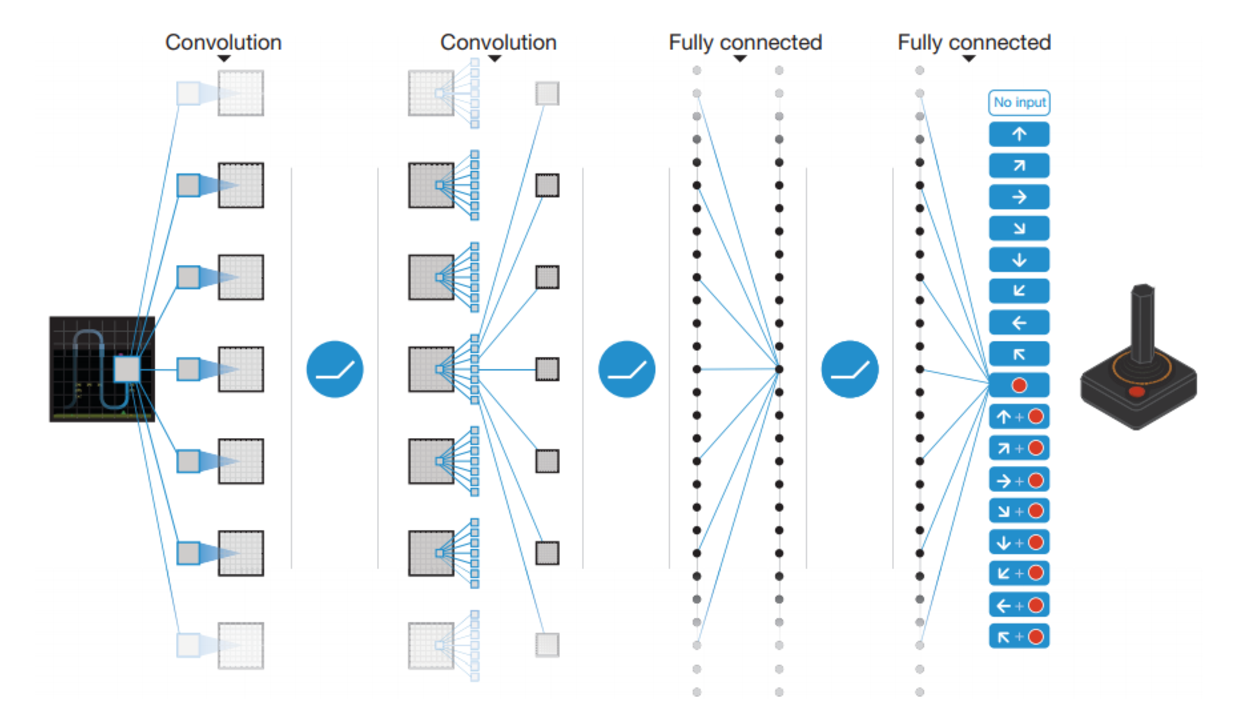
\includegraphics[width=0.8\textwidth]{Cap2/dqn.eps}
	\caption{Human level control through deep reinforcement learning in atari games
		\cite{mnih2015humanlevel}.}
	\label{dqn}
\end{figure}

With the advent of Deep Learning and its new techniques and the development of new computer architectures such as GPUs and TPUs, reinforcement learning has been able to scale as well, surpassing top players from the best table games. For example, the AlphaGo \cite{alphago} won against the human top player of Go, considered the hardest tabular game. It used a Monte-Carlo Tree Search with a Deep Neural Network to find a optimal policy through self-play and without any human knowledge. The evolution of AlphaGo, called AlphaZero \cite{alphazero} was able to learn not just Go, but also Chess and Shogi within a couple of hours.

On the other side, all the tasks mentioned before have discrete state or action spaces. The problem of kick motion involves continuous control. In this kind of problem, there's no discrete actions, but a interval of them. Therefore, the algorithms are different and must satisfact new optimization challenges.

In the last years, several algorithms arised in order to improve the performance in control tasks. These algorithms are commonly evaluated in the MuJoCo environment \cite{mujoco}, the most famous benchmark for continuous control tasks. Among such methods, we highlight A2C \cite{a2c}, ACER \cite{acer}, DDPG \cite{ddpg}, GAIL \cite{gail}, HER \cite{her}, TRPO \cite{trpo} and PPO \cite{ppoalgorithm}. The TRPO and PPO algorithms will be covered in deep later, and the last one will be used in the learning framework proposed in this work, since it has proved to perform better in the MuJoCo benchmark.

In terms of applications, \citeauthor{DBLP:journals/corr/HeessTSLMWTEWER17} applied a distributed variation of PPO in MuJoCo and were able to learn parkour movements and run in a model free fashion. These motions, however, are weird, asymmetric and, sometimes, unstable. \citeauthor{peng2018} applied the same algorithm but with key modifications in the reward function and optimization process, resulting in better and more human motions.

The most recent and impressive application of PPO was in OpenAI Five \cite{openaifive}. It consists of five independent neural networks that form a team to play the online game Dota 2. This team was trained in the equivalent of 180 years of continuous self-play, using 256 GPUs and 128 thousand of CPUs, and won from the $99.95^{th}$ percentile human team in a restricted environment. This is impressive not just because the environment is challenging -- due to the partial observability, long time horizon and high-dimensional, continuous spaces -- but also because of the multi-agent strategy layer learned. The network architecture used by OpenAI Five is shown in Figure \ref{openaifive}.

\begin{figure}[ht!]
	\centering
	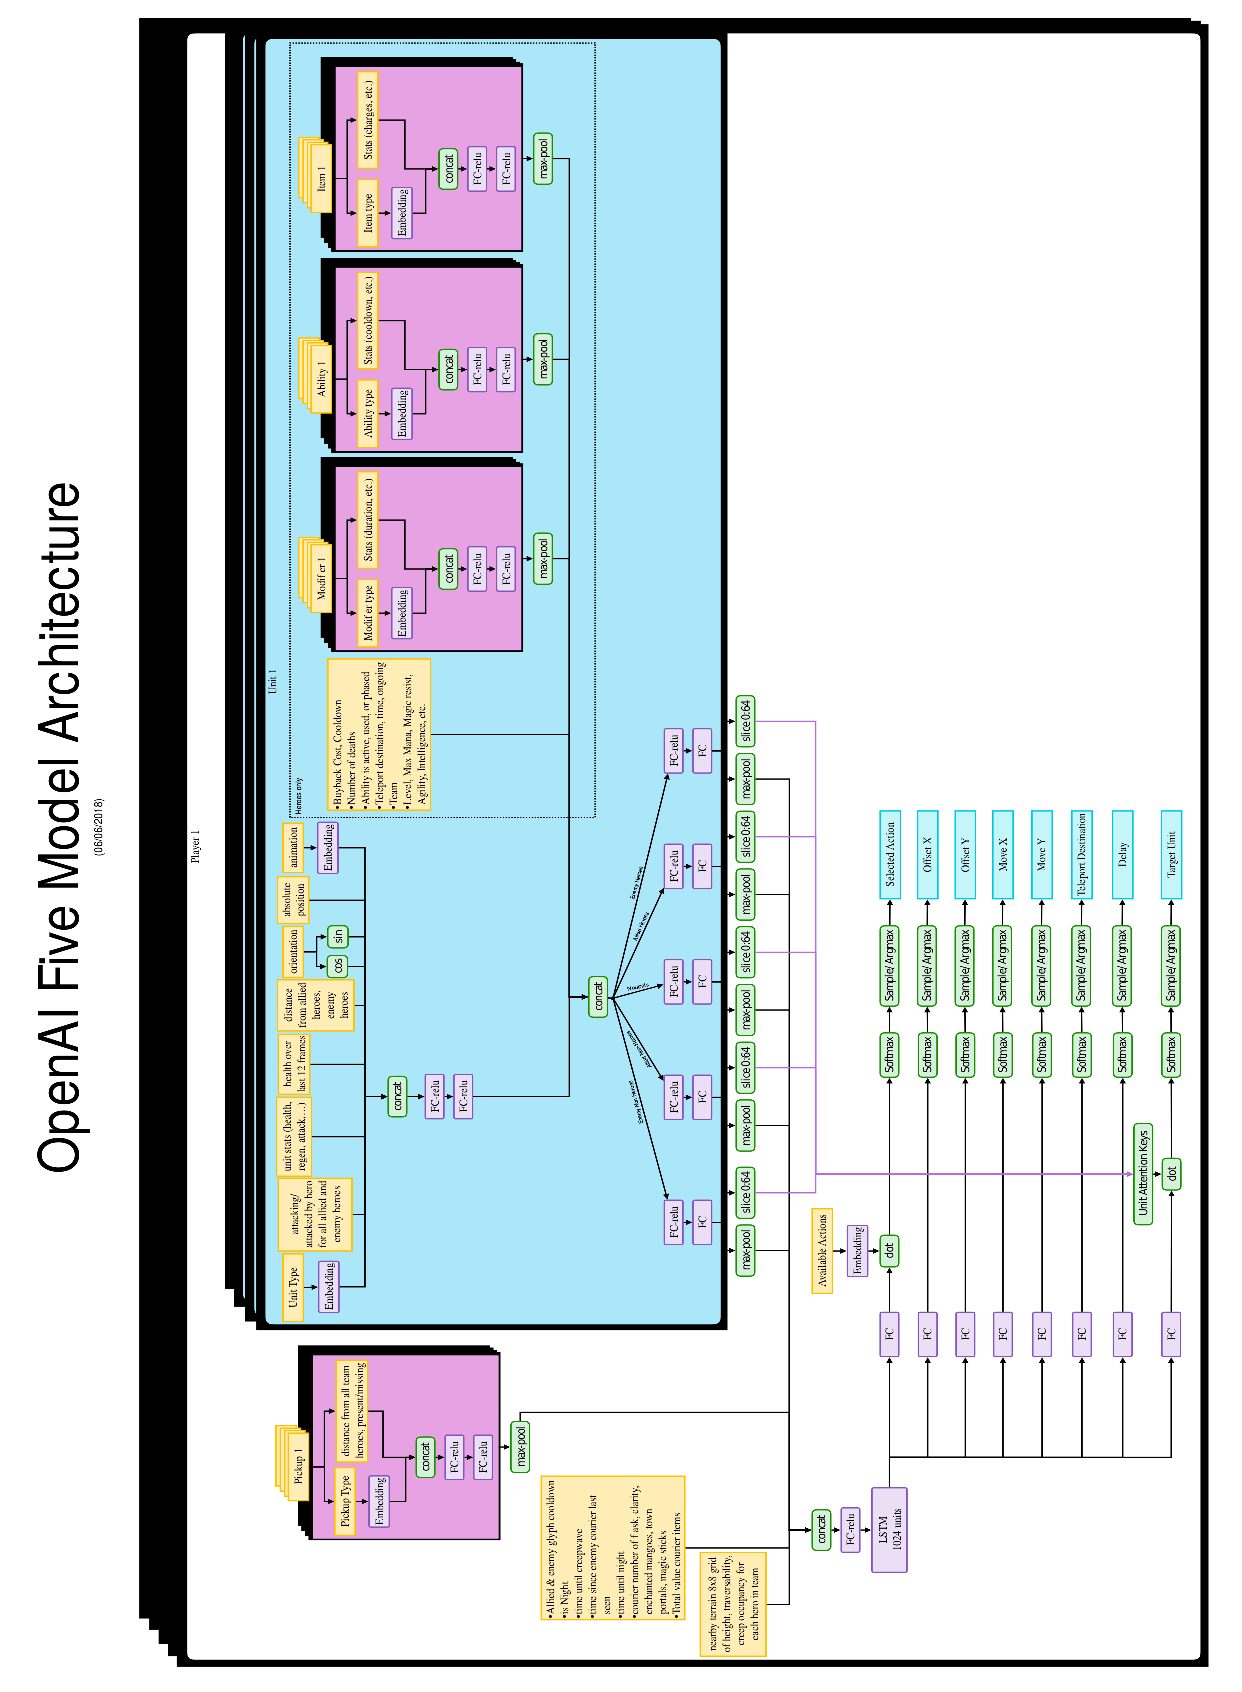
\includegraphics[scale=0.8]{Cap2/openaifive.eps}
	\caption{OpenAI Five network architecture \cite{openaifive}.}
	\label{openaifive}
\end{figure}

